\chapter{Searching for the best existing solution}\label{chapter:search}
Three-part composition is much richer than two-part composition. In fact, it offers many more possibilities than the two-part composition. In constraint solver terms, this means that the search space is much larger, which means two things: the computational complexity of finding a solution is greater, and there are many more possible solutions. The first difficulty is to find a valid solution in this large search space, and the second difficulty is to find the solution that best respects the preferences expressed by Fux.

In this chapter, we first discuss the computational aspect and then turn to the preference management aspect.
The computational complexity section covers: the search algorithm used, the heuristics implemented, and some of the factors that influence the speed of finding a solution; whereas the preference management section covers: discussing how to translate Fux's preferences into solver costs, and comparing the different methods that exist for doing so. 

\section{Dealing with the higher computational complexity}
As we have just said, composing a three-part counterpoint is more computationally demanding than composing a two-part counterpoint. The search space has been greatly expanded by adding a whole new set of variables, and the time it takes to find a solution may be too high if you do not think about optimising the search. In addition, adding a third voice to a composition does not bring many new constraints (which would help to discard some potential solutions faster), but it does bring many preferences, which in constraint programming are translated into costs. The solver must be efficient in finding the solution that has the lowest cost (i.e. that is best in terms of musicality).

\subsection{Using Branch-And-Bound as a search algorithm}

To cope with the increased complexity brought about by the three-part composition, it was decided to switch from the Depth First Search algorithm (used in T. Wafflard's thesis) to a more efficient Branch and Bound (BAB). This allows us to handle costs properly and to find faster solutions. Moreover, the BAB algorithm can also produce non-optimal results, which is very valuable since finding the best overall solution can be time-consuming. When starting the search for a solution, it is now possible to ask for the next solution (i.e. a better solution than the one found previously, and if none was found previously, then just any valid solution), or for the best solution. In the latter case, the solver will continue to search until it finds the best solution or until it is stopped, returning a better solution each time it finds one.


\subsection{Heuristics} \label{heuristics}
\subsubsection{Main heuristics}
When it comes to finding a solution, we obviously need some heuristics to guide the search, because there are so many different possibilities for a three-part composition. 
To know which heuristics to use, simply think about the most important variable to fix first. In case it is not clear enough, the key to writing counterpoint for many voices is to know what the bass is doing. This is true whether the composer is a human or a constraint solver. So the first heuristic follows naturally, and it is: branch on the lowest stratum array, take the highest constrained variable yet, and try with any value less than the median. This value branching was thought of because the possible values for the lowest stratum are those of the notes of the three parts. Since the lowest stratum is designed to always be equal to the lowest sounding note, it doesn't make sense to try to give it a high value. Therefore, lower values are chosen.


The other central heuristic is the one that instructs the solver to branch on the variables of the $N$ arrays (containing the pitches of the voices), choosing as a priority the variables whose domain is small. This choice is motivated by the fact that in the case of a highly constrained counterpoint (5th species) and a weakly constrained counterpoint (1st species), the counterpoint should not only seek to improve the highly constrained counterpoint, but also the weakly constrained counterpoint. This is why the heuristic chosen is based on the size of the domain and not on the level of constraint. The choice of the value of the variable is then random. This ensures maximum diversity in the final composition and quickly leads to a solution whose notes are varied.


\subsubsection{Additional heuristics}
A first additional heuristic is to branch to the array representing the species contained in the fifth species, to ensure a varied composition. If we are dealing with a counterpoint of the fourth or fifth species, we also branch on the "no ligature cost", so that the solver explores solutions in which the notes are linked, since this is the very nature of the fourth species (both when it is used "pure" and when it is used within the fifth species).

The rule~\ref{rule:start-distant} states that the voices should start distant, and as suggested in the section on rules, this should be implemented in a heuristic. However, when we implemented the heuristic that all voices should start distant from the lowest one, we did not see any improvement, neither in search speed nor in solution quality. In fact, it sometimes slowed down the search, so this heuristic was dropped. Furthermore, Fux's advice that the voices should start far apart in order to progress in the opposite direction is only true if the bottom layer moves up. If the bottom stratum moves down, the top strata should move up, so starting far apart becomes a compositional disadvantage in this case (as the voices are limited by their range).



\subsection{Time to find a solution} \label{section:time-to-find-a-solution}
Many factors come into play in determining how long it will take the solver to find a valid solution. These factors are mainly: the species of counterpoints, and the spacing between the voice ranges of the counterpoints.


In general, the solver is able to find a valid solution fairly quickly (in the order of a second). However, in some cases it is more difficult to find a valid solution and the solver may take a little longer to find one. These cases are generally related to the three factors mentioned above, and we will discuss them a little. Each of these factors makes the search a little more difficult. A single factor may have no effect on the search time, and sometimes it is at the intersection of the factors that an effect is discovered.

\begin{itemize}
    \item \textbf{Species of the counterpoint} \textendash{} The more complex the species of the counterpoints (think of the 3rd and 5th species, for example), the longer it will probably take the solver to find a solution. The reason is quite obvious: the more complex the species, the more variables the solver has to play with and the greater the range of possibilities.  
    \item \textbf{Distance between the voice ranges} \textendash{}  The closer the ranges of the voices, the greater the risk that the solver will take a long time to find a solution. For example, finding a solution by giving the two counterpoints the same voice range as the \cfs is more time-consuming than selecting distant voice ranges. This is because the voices cannot form a unison, and the possibilities for each voice are therefore smaller when their range is close together. 
\end{itemize}
There are also cases where the exact combination of two given vocal ranges for two given species with a given mode does not give a solution, but by changing the vocal range a little the solver finds a solution immediately, quite surprisingly. It is still unclear why this happens. Our best guess is that there are some combinations of parameters for which the solver has difficulty finding a solution, given the very large number of constraints that apply to the voices. However, this doesn't happen very often.

It is worth noting that the solver's greatest difficulty (in all cases) is finding a valid solution. Once a valid solution has been found, the solver quickly finds a whole series of solutions, each one better than the previous one (until, of course, it is difficult to find the best solution: then the solver starts taking some time again). The distance between the best solution and the solution found by the solver before reaching a plateau in the search is difficult to estimate. However, it should be remembered that the tool is intended to be used iteratively (the user tries a combination, changes the cost, tries again, etc.), and that in the end it is the user's human preferences that count, and there is no guarantee that the best solution will be the one the solver thinks is best. This means that it is the direction the solver takes that is important, not the best solution.


\section{Designing the costs of the solver to be as faithful as possible to the preferences of Fux} \label{costs}
A constraint solver cannot say whether one valid solution is better than another valid solution, and yet we need it to produce the best possible musical solution. We can already say that one solution is better than another if it respects Fux's preferences (see~\ref{subsection:preferences-vs-hard-rules}) more. In order for the solver to understand these preferences and to be able to distinguish the musical quality of two solutions, we give costs to it.  The lower the cost, the higher the preference.

Knowing that we are looking for the solution whose cost must be as low as possible, the question arises: how can we calculate the cost in order to best reflect the preferences expressed in \gap?

The way to translate each preference into a corresponding cost has of course been formalised in the previous sections, but that's not the crux of the matter. The question we face here is: what is the best way to combine all these individual costs to get the most accurate result in terms of what Fux is trying to convey in terms of preferences?

Three main ways of doing this have been identified. These are, in order from the simplest to the most complex:
\begin{enumerate}
    \item a linear combination of all costs,
    \item computing the maximum over all costs and minimising it,
    \item a lexicographic order search, 
\end{enumerate}
We first describe each of these techniques and their respective advantages, and then compare them (and the results they produce).

Throughout this section we talk about some specific costs. All these costs are listed in~\ref{fig:default-order-lexico} with a short explanation. Some more details can be found in~\ref{appendix:interface-parameters-description}, and for the full description of a specific cost, please refer to its corresponding rule. 


\subsection{Linear Combination}


The first method of calculating our costs is a linear combination. This is the technique used in T. Wafflard's thesis. More precisely, it uses a linear combination in which all the weights are equal to one.



To be more precise about the method used to calculate the total cost in T. Wafflard's thesis, here is a more detailed explanation: there exists a total cost, $\tau$, which is equal to the sum of all individual costs, $\mathcal{C}$. The next step is to minimise $\tau$. Each $\mathcal{C}_i$ is usually itself a sum of sub-costs. Take, for example, the cost of motions, $\mathcal{C}_{motions} = \sum_j P_{costs}[j] $. This cost is the sum of all sub-costs of the motions (one per motion): by default, a contrary motion has a sub-cost of 0, an oblique motion has a sub-cost of 1 and a direct motion has a sub-cost of 2. These default values can be changed by the user to be set somewhere on a scale that ranges from $0$ to $64m$. For example, the user could set the oblique motion cost to be equal to $0$, and the cost for direct and contrary motion to be equal to $64m$, in order to get a composition filled with as many oblique motions as possible (always in accordance with the basic rules from \gap, i.e. all voices are never going to go in the same direction, see~\ref{rule:same-movement}).

As mentioned at the beginning of this subsection, this procedure can be understood as a linear combination with weights of one only. However, since the cost factors are given different values according to the user's choices, this method is actually more like a regular linear combination, except that the weights are not multiplied by the costs once the latter have been set, but the costs are themselves made larger or smaller before the linear combination is calculated.

\paragraph{}
The linear combination has two major advantages: ease of implementation and high comprehensibility.
However, it has a major drawback: since the total cost $\tau$ that gets minimised is the sum of all costs $\mathcal{C}$, the best solution might be a solution where one cost is absolutely huge and all the others are small. This might not be a problem if the outstanding cost is not really relevant, but if it is the cost of not using a harmonic triad, it goes completely against the preferences that Fux conveys in his work, making the solution inappropriate. A representation of this situation can be found in the figure~\ref{fig:outstanding-cost}.

\begin{figure}[h!]
    \centering
    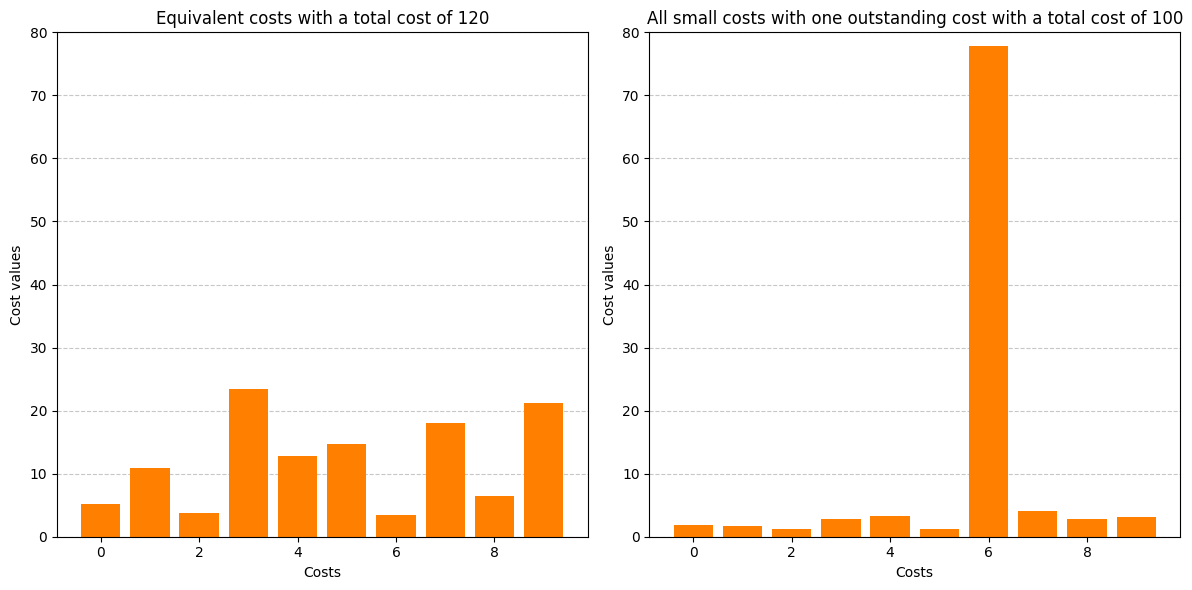
\includegraphics[width=1\textwidth]{Images/outstanding-costs.png}
    \caption{Example of a situation where a solution with an outstanding cost is preferred to a solution with equivalent low costs when using a linear combination}
    \label{fig:outstanding-cost}
\end{figure}

Another disadvantage of linear combination is that the result is quite unpredictable: changing the value of the cost may or may not make a difference, and you may need to set huge values to see a real effect. For example, if a composer really wants oblique motion, they may be forced to set the cost of the other types of motion to a huge value, or they may not see the difference between the default solution and their personalised solution. This is due to the fact that all the costs are mixed together and form an indistinguishable soup that the solver considers as a whole, and a small increase in the cost of the direct and contrary motions is very likely to be absorbed into this soup without any change being noticed.

These two drawbacks make the linear combination solution for the costs hardly acceptable when it comes to representing the preferences.
We therefore examine the other two options for adjusting costs.

\subsection {Minimising the maxima} \label{section:minimising-the-maxima}
In order to overcome the problem of outstanding costs that we encountered when considering the linear combination solution, one could consider a technique that specifically addresses these outstanding costs: namely, minimising the maximum cost.For example, $\tau$ the total cost, could be set equal to the current largest cost. By doing this, the solver would try to find a solution where the focus is on the worst cost and try to reduce it before trying to reduce the other costs.

The problem with this method arises when one cost is significantly higher than the others because it has been defined that way. Let's go back to our example of the composer wanting as many oblique motions as possible. You will set the cost for direct motion and contrary motion to the highest possible cost and start the search. As we've already discussed, it is not possible to have only oblique motions, since this would contradict the rule that not all voices can move in the same direction (\ref{rule:same-movement}). As a result, there will always be contrary motions, and since the cost for them has been set very high, it would be impossible for the solver to converge to a good solution. This creates a bottleneck effect, where once the solver has reached the best potential value of the worst cost, it cannot continue to find better solutions. 

\begin{figure}[h]
    \centering
    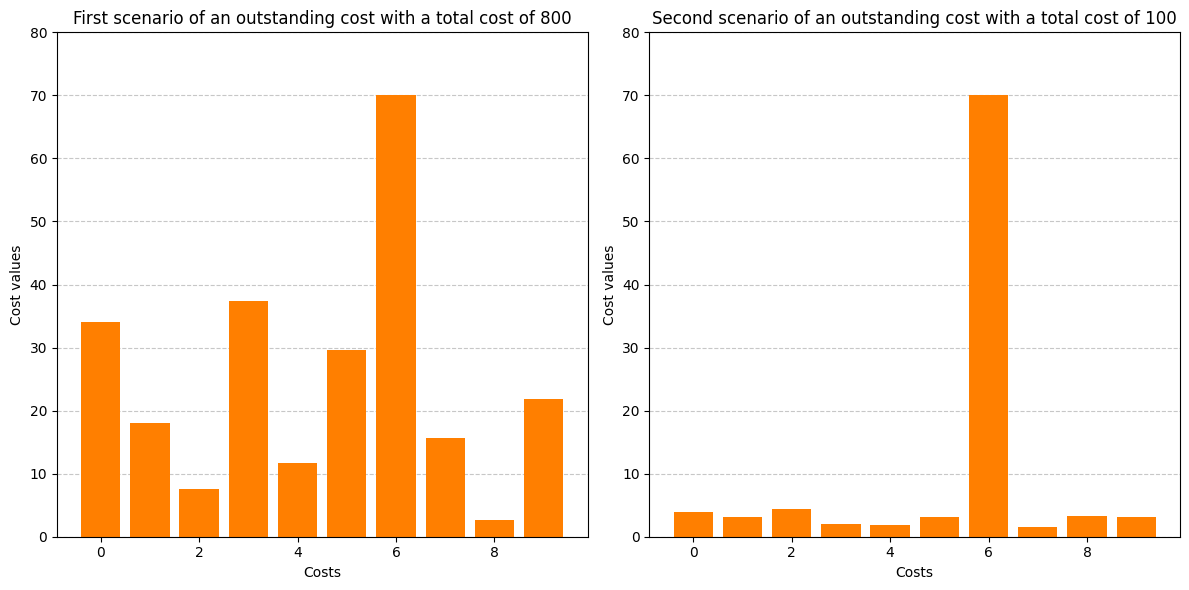
\includegraphics[width=1\textwidth]{Images/minimising-maxima.png}
    \caption{Example of two situations where a cost causes a bottleneck in the search because the solver cannot distinguish between left and right situations. The solver will blindly choose one of the two solutions, even if the solution on the left is obviously better.}
    \label{fig:bottleneck}
\end{figure}


Furthermore, even when considering a less extreme case (e.g. the default setting), this method requires a normalisation of the costs: there are $3\times (m-2)$ sub-costs for the variety cost, $3\times (m-1)$ sub-costs for the motion cost, but only $m$ sub-costs for the octave cost. This means that without normalisation, the motion cost will be on average three times larger than the octave cost, which means that the solver will put three times more effort into minimising the motion cost than the octave cost, which is unfair and unpractical.


\subsection{Lexicographic Order}\label{section:lexicographic-order}
The second way of dealing with the costs is to arrange them in an array and then perform a lexicographic minimisation. In other words, the costs would be arranged in order of importance: from most important to least important. The most important cost to minimise would be placed first in this array, and the solver would only try to minimise the other costs if the first cost remained the same or decreased. This method makes a lot of sense when you think about the rules that emanate of \gap. For example, Fux says that perfect consonance can be achieved by direct motion if there is no other possibility. This means that, all other things being equal, we would prefer to achieve perfect consonance by oblique or contrary motion, but that between a bad solution (respecting almost no preferences) in which perfect consonance is not achieved by direct motion, and a good solution (respecting almost all preferences) in which perfect consonance is achieved by direct motion, we would choose the good solution. 

Some costs are also more important than others in absolute terms. For example, when Fux says that an imperfect consonance is preferred to a fifth, which is preferred to an octave. This amounts to lexicographicly ranking the cost of using an octave first (because we really don't want octaves), and then the cost of using a fifth (and there is no cost of using an imperfect consonance, since Fux indicates that this is preferable).
\begin{figure}[h]
    \begin{equation}
        \begin{aligned}
            \tau = [\underset{\text{minimise this first}}{\underbrace{\mathcal{C}_\text{octaves}}}, \mathcal{C}_\text{fifths}]
        \end{aligned}
    \end{equation}
    \caption{Array of costs demonstrating the practicality of a lexicographic order solving.}
\end{figure}

A second example, which ties in particularly well with the first, is that Fux tells us that the harmonic triad must be used in every measure unless a rule forbids it. In saying this, he places the preference for the harmonic triad above all other preferences, because the only reason that can prevent the use of a harmonic triad is a fixed constraint (and not a preference). You'll notice that the harmonic triad consists of a fifth (which is a perfect consonant), so Fux is telling us that we'd rather use a fifth in a harmonic triad than an imperfect consonant outside a harmonic triad. The lexicographic order search is the only one that allows this kind of concept to be taken into account, because in a linear combination these two preferences would be mutually "exclusive"\footnote{In the sense that their effects would work against each other.}: the first preference would add a cost where the second preference would not, and the second preference would add a cost where the first would not.

\begin{figure}[h]
    \begin{equation}
        \begin{aligned}
            \tau = [& \underset{\text{\fontsize{7}{11}\selectfont{minimise this first}}}{\underbrace{\mathcal{C}_\text{harmonic\_triad}}}, \underset{\text{\fontsize{7}{11}\selectfont\parbox{4cm}{and start minimizing this only if it is not possible anymore to minimise the harmonic triad cost}}}{\underbrace{\mathcal{C}_\text{octaves}}},\quad  \mathcal{C}_\text{fifths}]
        \end{aligned}
    \end{equation}
    \caption{Array of costs demonstrating the practicality of a lexicographic order solving.}
\end{figure}

And in this way we can keep integrating the different costs until we get a full array $\tau$ with all the costs ordered in a lexicographic way.


Of course, it is not always as simple as in the examples above, because it is not always easy to determine which cost has priority over which other. Sometimes Fux is very clear about it (e.g. for the harmonic triad cost, which Fux says has priority over everything else), and sometimes he isn't (do we prefer no off-key notes, or as much variety as possible?) This is a drawback of this method, because we have to hierarchise the costs, even if the choice is difficult. What's more, once the costs are ranked, their order becomes absolute and the solver loses some of its flexibility.


Knowing this, we came up with a suggested order that should be as close as possible to Fux's preferred order (or at least what we understood him to convey as his preferred order in \gap). This order should of course be changeable at the composer's discretion\footnote{Please have a look at Appendix~\ref{chapter:user-guide} to see how the composer can personalise the order.}. The default order we have agreed upon is as follows. Please note that where a cost is followed by a number in brackets, this means that it only applies if the corresponding species is used.
\begin{multicols}{2}
    \begin{enumerate}\label{fig:default-order-lexico}
        \item $\mathcal{C}_\text{no\_syncope}$\footnote{The cost of not using a syncope.} [4, 5] 
        \item $\mathcal{C}_\text{successive\_p\_cons}$
        \item $\mathcal{C}_\text{harmonic\_triad}$
        \item $\mathcal{C}_\text{harmonic\_triad\_3rd\_species}$ [3]
        \item $\mathcal{C}_\text{octaves}$
        \item $\mathcal{C}_\text{penult\_thesis\_is\_fifth}$\footnote{A specific cost for the second species, which applies when a penultimate thesis note does not make a fifth interval with the lowest stratum.} [2]
        \item $\mathcal{C}_\text{fifths}$
        \item $\mathcal{C}_\text{off\_key}$\footnote{The cost of using sharps or flats.}
        \item $\mathcal{C}_\text{variety}$
        \item $\mathcal{C}_\text{m2\_eq\_zero}$\footnote{The cost of having the same note in the downbeat and the upbeat.} [3, 4, 5]
        \item $\mathcal{C}_\text{not\_cambiata}$\footnote{The cost of not using a \textit{cambiata} if it is possible. The \textit{cambiata} can be characterised by the following scheme: \texttt{consonance - dissonance - consonance}.} [3, 5]
        \item $\mathcal{C}_\text{motions}$
        \item $\mathcal{C}_\text{m\_degrees}$\footnote{The cost of using big or small melodic intervals.}        
        \item $\mathcal{C}_\text{direct\_move\_to\_p\_cons}$
    \end{enumerate}
\end{multicols}

Some notes on the proposed order: 
\begin{itemize}
    \item Two costs come even before the harmonic triad cost: the $\mathcal{C}_\text{no\_syncope}$ cost and the $\mathcal{C}_\text{successive\_p\_cons}$ cost. Regarding the $\mathcal{C}_\text{no\_syncope}$ cost: this cost is at the heart of the fourth species, and a fourth species counterpoint without syncopations is not really a fourth species counterpoint. This is why syncopation is considered even more important than the harmonic triad. And concerning the $\mathcal{C}_\text{successive\_p\_cons}$ cost: when Fux expresses his preference for the harmonic triad, he says that there are reasons that are even more important (see rule~\ref{rule:harmonic-triad}), and not having successive perfect consonances is one of them.
    \item The cost of $\mathcal{C}_\text{penult\_thesis\_is\_fifth}$ comes before the cost of $\mathcal{C}_\text{fifths}$, as it is an exception to the latter (similar to the interaction explained above in the section between $\mathcal{C}_\text{harmonic\_triad}$ and $\mathcal{C}_\text{fifths})$.
    
    \item $\mathcal{C}_\text{off\_key}$ was added to its ranking because it is actually an absolute rule not to use off-key notes, but Fux does use some, and so it was decided to put this cost after the very important costs to allow off-key notes to happen.

    \item The costs $\mathcal{C}_\text{variety}$, $\mathcal{C}_\text{motions}$ and $\mathcal{C}_\text{m\_degrees}$ were ranked in order from least to most restrictive. First we say that we would prefer the note to change as much as possible (with the variety cost), then we indicate our preference for the direction (with the motion cost), and finally we indicate our preference for the size of the motion (with the melodic interval cost). This gives the solver as much flexibility as possible. The other way round would have been more restrictive, since the solver would have minimised the melodic intervals first, setting them all to one, which doesn't leave much room for the motion cost to have an effect, and forcing the variety cost to be high in any case, as with  intervals the melody tends to vary only a little.
    
    \item $\mathcal{C}_\text{m2\_eq\_zero}$ and $\mathcal{C}_\text{m\_degrees}$ were classified right after the variety cost as they are an in-measure variation of the variety preference.

\end{itemize}


\paragraph{NB} Please note that using the lexicographic order does not \textit{not} mean that the last costs are not taken into account, they will be \textit{too} minimised by the solver. It just means that if the solver has to choose between minimising one cost or another, it will minimise the first one in the lexicographic order. 

\subsection{Comparison between the three types of costs.}

We have now discussed the advantages and disadvantages of each of the three methods. These are all listed in Table~\ref{tab:comparison}. As you can see, no one method is definitively better than another, and the only way to know which method is better in practice is to \textit{test} them in practice to find out which of the methods gives the best results. 
\newpage
\begin{center}
    \centering
    \captionof{table}{Comparison of Three Methods According to Criteria}
    \label{tab:comparison}
    \begin{tabularx}{\textwidth}{|>{\centering\arraybackslash}p{4cm}|>{\centering\arraybackslash}X|>{\centering\arraybackslash}X|>{\centering\arraybackslash}X|}
        \hline
        \textbf{Criteria} & \textbf{Linear Combination} & \textbf{Minimising the maximum} & \textbf{Lexicographic Search} \\
        \hline
        Outstanding costs & \cellcolor{red!25}Yes & \cellcolor{green!25}No & \cellcolor{orange!25}Only for minor costs \\
        \hline
        Sensitivity\footnote{In the sense that changing one cost has a big impact on the result.} & \cellcolor{red!25}No & \cellcolor{orange!25}Some & \cellcolor{green!25}Yes \\
        \hline
        One cost might be a bottleneck & \cellcolor{green!25}No & \cellcolor{red!25}Yes & \cellcolor{green!25}No \\
        \hline
        Need to normalise costs& \cellcolor{green!25}No & \cellcolor{red!25}Yes & \cellcolor{green!25}No \\
        \hline
        Possibility to ensure a preference of one cost over another  & \cellcolor{red!25}No & \cellcolor{red!25}No & \cellcolor{green!25}Yes \\
        \hline
        Need for hierarchisation of costs & \cellcolor{green!25}No & \cellcolor{green!25}No & \cellcolor{red!25}Yes \\
        \hline
        Flexibility & \cellcolor{orange!25}Medium & \cellcolor{green!25}High & \cellcolor{red!25}Low \\
        \hline

    \end{tabularx}
\end{center}

Even more, one could think about a combination of all the methods to get rid of their disadvantages. In fact, we could enjoy the advantages of all the methods by combining them and cleverly designing a lexicographic order search in which the cost is a linear combination of a maximum minimisation.

\section{Experimenting with the three types of costs arrangement}
To experiment which method gives the best results, we will follow this plan: first compare the result of a linear combination and the result of a purely lexicographic order, using the default preference order as defined in~\ref{section:lexicographic-order}. We then analyse the result by looking at what could have been done to manage costs more effectively and, where appropriate, group costs together.

These experiments are carried out using different counterpoint combination setups. These setups will increase in complexity, starting with the basic case of 3-voice counterpoint (two counterpoints of the 1st species) and moving on to mixed counterpoints. 

The advantage of simple species (first, second and fourth species) is that the search for a solution is much faster. In fact, the search for an optimal solution can be quite time-consuming, and this is even more the case when we are talking about complex species such as the third and the fifth, and when they are combined. This means that it is more difficult to grasp the impact of the cost method when using a setup with complex species. What's more, the vast majority of the costs are related to the interaction of the voices in the first beat of the measures: the behaviour we want to observe, i.e. the interaction between the cost method and the resulting composition, will be just as observable with complex species as with simple ones. Having said that, we are still going to test the cost arrangement methods on all species.

The analyses in this section are superficial and do not deal with in-depth music theory. They will consist of general surface and impression remarks. They are highly subjective and should not be taken at face value. The aim of this analysis is to provide an initial critical view of the results offered by the solver.

The selected \textit{cantus firmi} were chosen from \gap. 
\subsection{Comparing the linear combination and the lexicographic order in practice}
\subsubsection{First experiment: two first-species counterpoints on two different \textit{cantus firmi}}
For this first experiment, if the search time exceeds 30 seconds, the search is stopped and the current solution is analysed.
\begin{figure}[h]
    \centering
    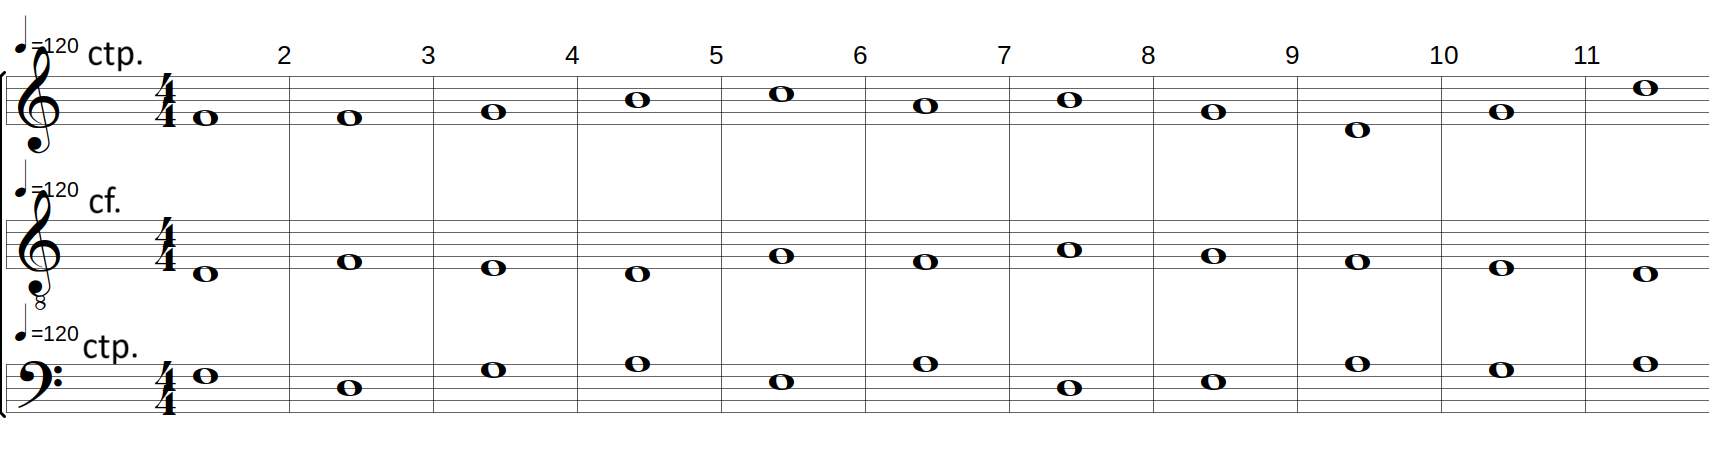
\includegraphics[width=1\textwidth]{Images/Experiments/linear-combination-1sp.png}
    \caption{Result 1 of the linear combination method with default costs. Click \href{https://youtu.be/w7EQ3b8JHnM}{here} to listen.}
    \label{fig:combili-1sp}
\end{figure}

\begin{figure}[h]
    \centering
    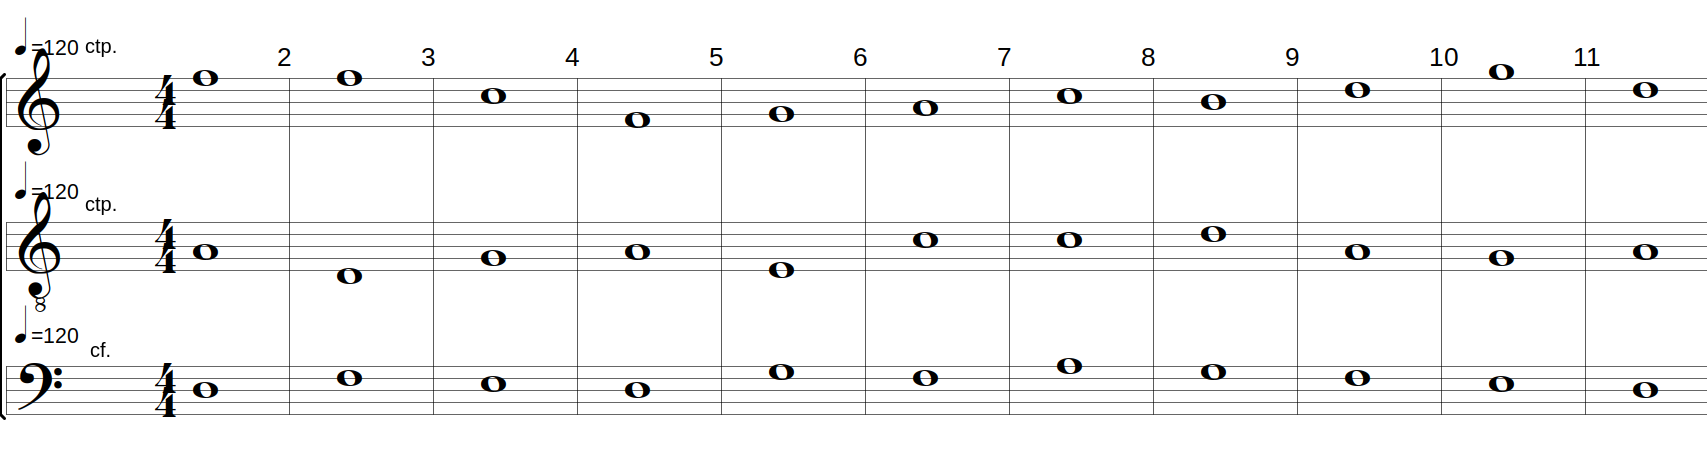
\includegraphics[width=1\textwidth]{Images/Experiments/basic-lexico-1sp.png}
    \caption{Result 1 of the lexicographic search method with default costs. Click \href{https://youtu.be/ryrpi5QNmf0}{here} to listen.}
    \label{fig:lexico-1sp}
\end{figure}

% above very far above
Here are the first two results:~\ref{fig:combili-1sp} and~\ref{fig:lexico-1sp}. To the average ear, there's not much difference between these two solutions.

In more technical terms, here are the cost arrays: 
\begin{itemize}
    \item for the linear combination: $[2, 20, 0, 3, 4, 6, 4, 14, 0]$, with a total sum of 53,
    \item for the lexicographical order: $[\underset{\text{succ\_p\_cons}}{\underbrace{0}}, \underset{\text{h\_triad}}{\underbrace{14}}, 0, 3, 0, 10, \underset{\text{motions}}{\underbrace{16}}, 14, \underset{\text{direct\_m\_p\_cons}}{\underbrace{8}}]$, with a total sum of 65.
\end{itemize}

As we can see, the difference between the two is exactly what we expected: high importance costs are prioritised and low importance costs are neglected in the lexicographic search, while the linear combination tries to minimise everything. A good example of this is the harmonic triads: they are more present in the lexicographic solution than in the linear combination (four versus one). Meanwhile, there are seven direct motions and two oblique motions in the lexicographic solution and only two direct motions in the linear combination solution\footnote{Please remember that the motions are computed with respect to the lowest sounding note.}.

\begin{figure}[h]
    \centering
    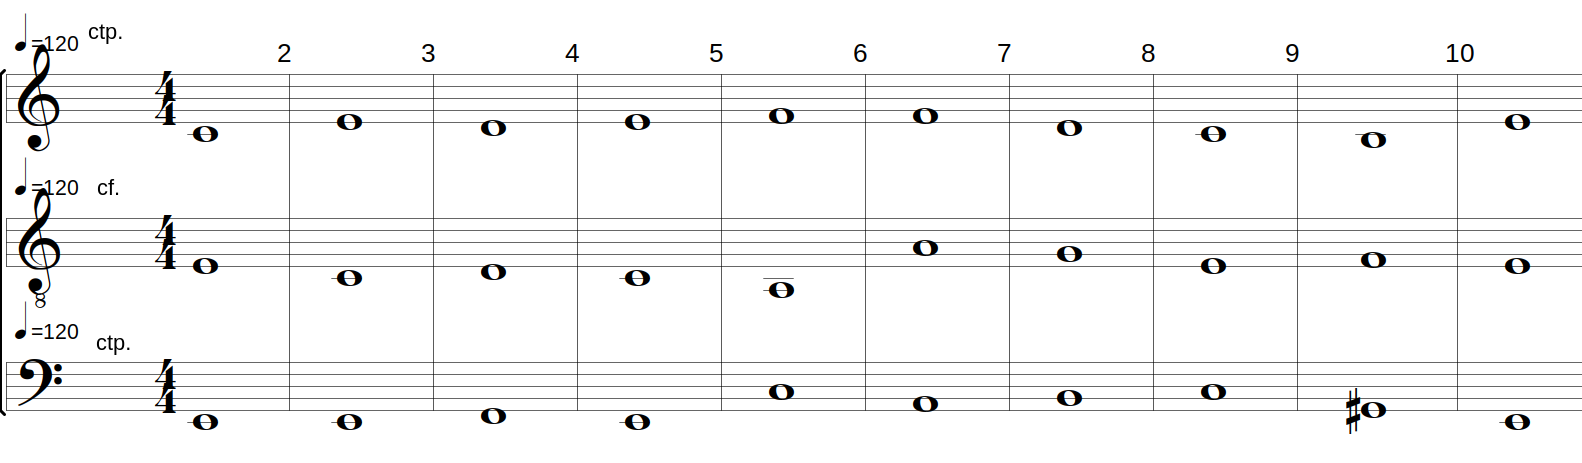
\includegraphics[width=1\textwidth]{Images/Experiments/linear-combination-1sp0.png}
    \caption{Result 2 of the linear combination method with default costs. Click \href{https://youtu.be/pnwceQyZd9E}{here} to listen.}
    \label{fig:combili-1sp0}
\end{figure}

\begin{figure}[h]
    \centering
    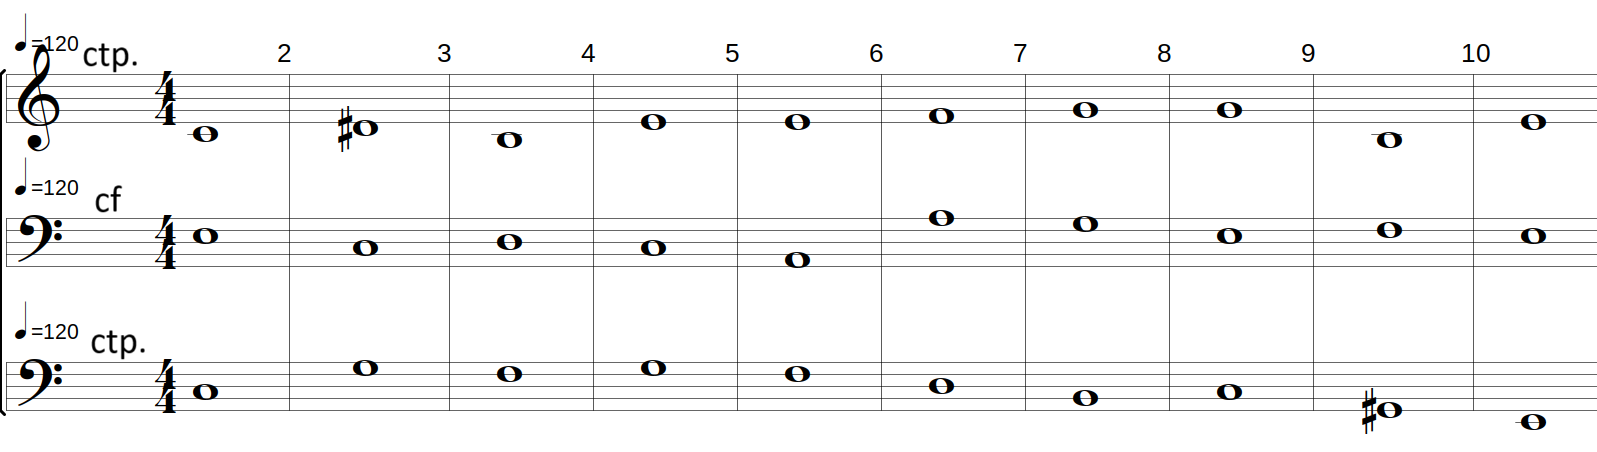
\includegraphics[width=1\textwidth]{Images/Experiments/basic-lexico-1sp0.png}
    \caption{Result 2 of the lexicographic search method with default costs. Click \href{https://youtu.be/-twWU-hNcYI}{here} to listen.}
    \label{fig:lexico-1sp0}
\end{figure}

% below far above
\paragraph{}
Let's look at the second result (obtained with a different \cf), featured in figures~\ref{fig:combili-1sp0} and~\ref{fig:lexico-1sp0}.
Once again, the technical results are fairly as one would expect them:
\begin{itemize}
    \item for the linear combination: $[0, 20, 4, 0, 4, 12, 11, 8, 8]$, with a total sum of 67,
    \item for the lexicographical order: $ [0, 16, 0, 2, 4, 8, 10, \underset{\text{melodic\_intervals}}{\underbrace{19}}, 8]$, with a total sum of 67.
\end{itemize}
For the average listener, it is difficult to establish an absolute preference between these two solutions.
We will take this same setting and try to mix the techniques for it in section \ref{subsection:mixing-the-techniques}.

\subsubsection{Second experiment: one fourth-species counterpoint and one first-species counterpoint on a single \cf}

If we now go on, here is a result combining the first and the fourth species, and putting the 4th species at the bottom:
\begin{figure}[h]
    \centering
    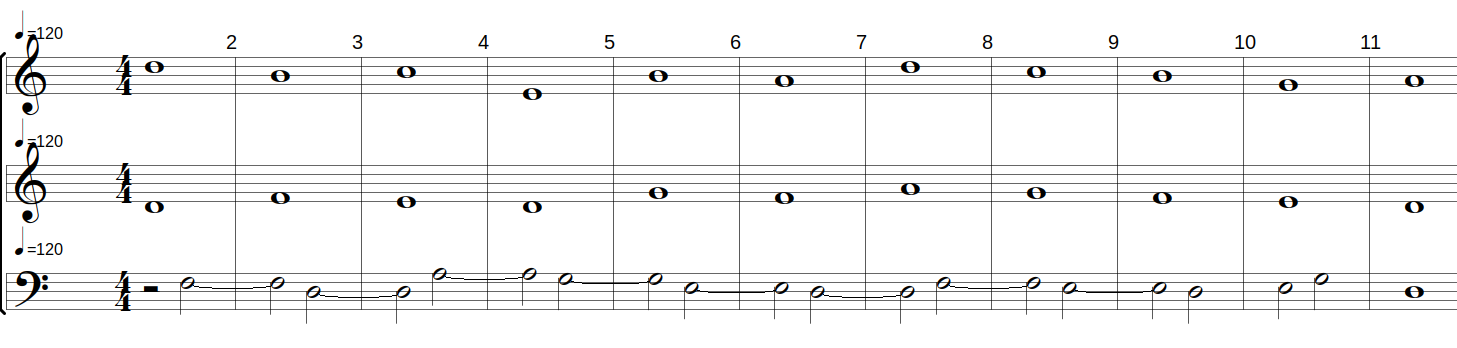
\includegraphics[width=1\textwidth]{Images/Experiments/linear-combination-4sp.png}
    \caption{Result 3 of the linear combination method with default costs. Click \href{https://youtu.be/eunaKHOQ2Nk}{here} to listen.}
    \label{fig:combili-4sp}
\end{figure}

\begin{figure}[h]
    \centering
    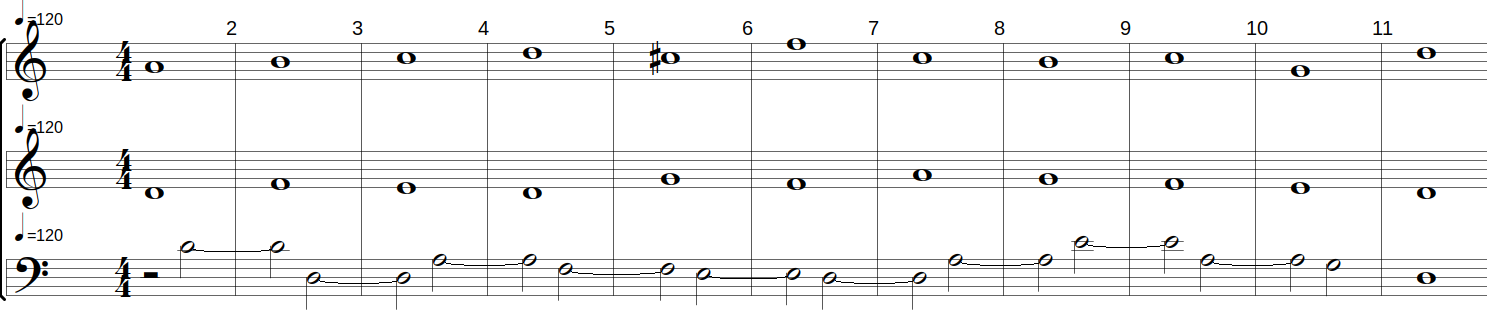
\includegraphics[width=1\textwidth]{Images/Experiments/basic-lexico-4sp.png}
    \caption{Result 3 of the lexicographic search method with default costs. Click \href{https://youtu.be/rh3YdRu62J4}{here} to listen.}
    \label{fig:lexico-4sp}
\end{figure}
Looking at the results obtained with this setup (figures~\ref{fig:combili-4sp} and~\ref{fig:lexico-4sp}), we come to the following conclusion: in both cases, the melody is a little dull and lacks dynamism. There is no drastic change in quality between the solutions provided by the two search techniques. However, the solution provided by the lexicographic search is somewhat more exciting, since there is more tension in it and it uses more dissonances and resolvings than the linear combination (even if these resolvings are not the most brilliant).

We immediately notice something else with the 4th species on the bass, which is not related to the costs: there are a few dissonances on the downbeat, as the solver doesn't really take into account the harmonic interaction between the notes of the downbeat of the fourth species and the notes of the downbeat of the other species, but rather the harmonic interaction between the upbeat of the fourth species and the downbeat of the others: which leads to a few surprises, as we can see in these examples (that tension mentioned above).

As far as the costs are concerned, one thing is clear: not all the notes of the 4th species obtained with a linear combination are linked, whereas they all are in the solution of the lexicographic order. This is an obvious consequence of using a linear combination, as this technique is not able to prioritise a cost.


\subsubsection{Third experiment: one third-species counterpoint and one second-species counterpoint on a single \cf}
Our first cross-species test will involve a counterpoint of the 2nd species and a counterpoint of the 3rd species. The \cfs used is the one proposed by Fux in an example in which he uses exactly these two species. The search was given one minute, as the complexity is getting higher than in the previous experiments. \label{subsection:third-experiment-with-costs}


The results are shown in the figures:

\begin{figure}[h]
    \centering
    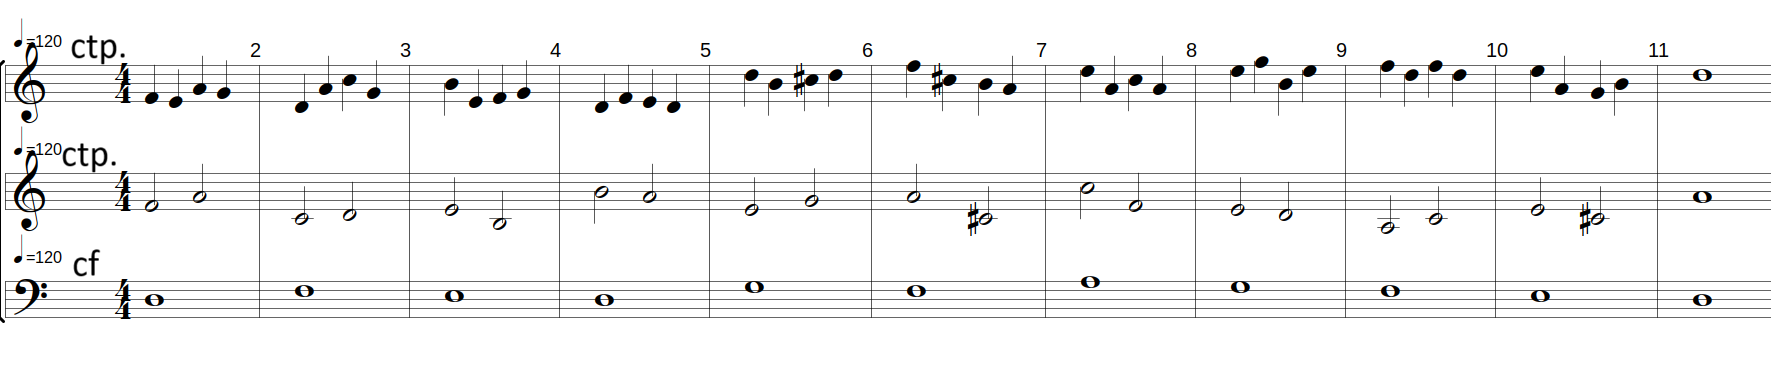
\includegraphics[width=1\textwidth]{Images/Experiments/linear-combination-2sp.png}
    \caption{Result 4 of the linear combination method with default costs. Click \href{https://youtu.be/_VrM76hp1v8}{here} to listen.}
    \label{fig:combili-2sp}
\end{figure}

\begin{figure}[h]
    \centering
    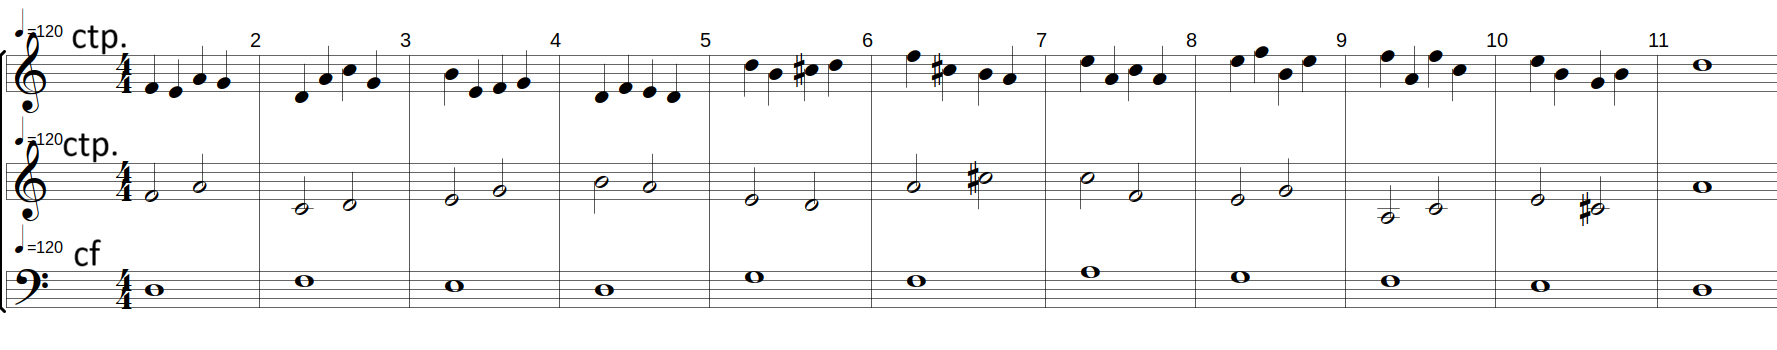
\includegraphics[width=1\textwidth]{Images/Experiments/basic-lexico-2sp.png}
    \caption{Result 4 of the lexicographic search method with default costs. Click \href{https://youtu.be/msY1LOGw3v8}{here} to listen.}
    \label{fig:lexico-2sp}
\end{figure}

The results are strikingly similar and quite unmelodic. Let's look at these two aspects in turn.

About the similarity: The similarity is probably due to two things: the solver doesn't have much room for manoeuvre, since all the voices are highly constrained, so the costs don't have much of an effect in this very setup. 

Concerning the lack of melodic quality: it is probably due in part to bad luck (this \cfs is perhaps particularly difficult to handle) and in part to the lack of constraints linking the upbeats of the various counterpoints. If you think about it, all the rules proposed by Fux in his chapter on three-voice composition link the beats of one voice (\textit{all its beats}) to the first beat of the other voices. This means that there are constraints between the 2nd, 3rd and 4th beats of one voice and the other voices, but never between these 2nd, 3rd and 4th beats of one voice and the 2nd, 3rd and 4th beats of another voice, always with the 1st beat. Obviously, without rules to ensure that the notes of these beats concur\footnote{The word 'concur' is used here in the same sense that Fux uses it: it means that the notes are somehow put in a relationship that makes them sound good together.}, it is more complicated for these beats to concur. Of course, it would be wrong to say that it depends only on chance that these beats concur, because that would mean that the beats are independent. Indeed, one might think so at first, because there are no constraints directly linking them, and yet they are linked by their own connections with the first beat of the other voices. In other words, although the third beat of the first counterpoint is not directly linked to the third beat of the second counterpoint, it is indirectly linked to it through the first beat of the second counterpoint: there are constraints between this third beat of the first counterpoint and the first beat of the second counterpoint, and there are also constraints between the first beat of the second counterpoint and the third beat of the second counterpoint. There is therefore a certain dependency and mutual influence between the 3rd beats of the two counterpoints. However, it would be interesting to see if Fux introduces any rules on this subject in his chapter on four-part composition, and if not, it would be interesting to think about what these rules might be in order to maximise the concordance between the notes in the upbeat of the different voices.
\subsubsection{Fourth experiment: two fifth-species counterpoints}
The fourth experiment is a bit special, as it features two fifth counterpoints \textit{with the same voice range}. This is something Fux doesn't really do in \gap, but we thought it might be interesting to see how the search method behaves in this situation. Even though Fux doesn't write counterpoints in the same voice range, they are still realistic, for example in the case of a double violin concerto, or any other instrument that has the same voice range and that is played together.

In this experiment, it is interesting to observe how the solver manages the small margin of manoeuvre it has, given that it has to find two counterpoints in the same voice range, all when the counterpoints are forbidden to take the same value (i.e. the same pitch).

The search was run for two minutes instead of thirty seconds, as the fifth species counterpoint is more complex than the others, and a little more time is needed to let the costs have an effect on the solution. The solutions are those in figures~\ref{fig:combili-5sp} and~\ref{fig:combili-5sp}.

\begin{figure}[h]
    \centering
    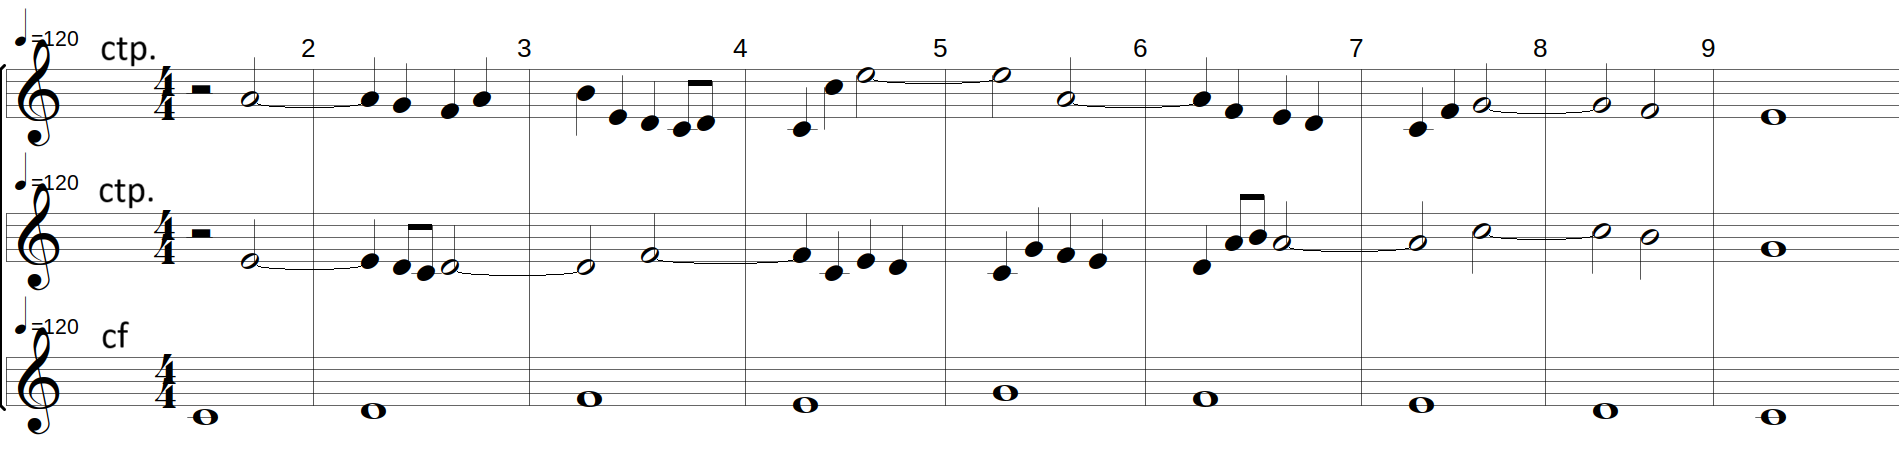
\includegraphics[width=1\textwidth]{Images/Experiments/linear-combination-5sp.png}
    \caption{Result 5 of the linear combination method with default costs. Click \href{https://youtu.be/Lyi2Tv0eto8}{here} to listen.}
    \label{fig:combili-5sp}
\end{figure}

\begin{figure}[h]
    \centering
    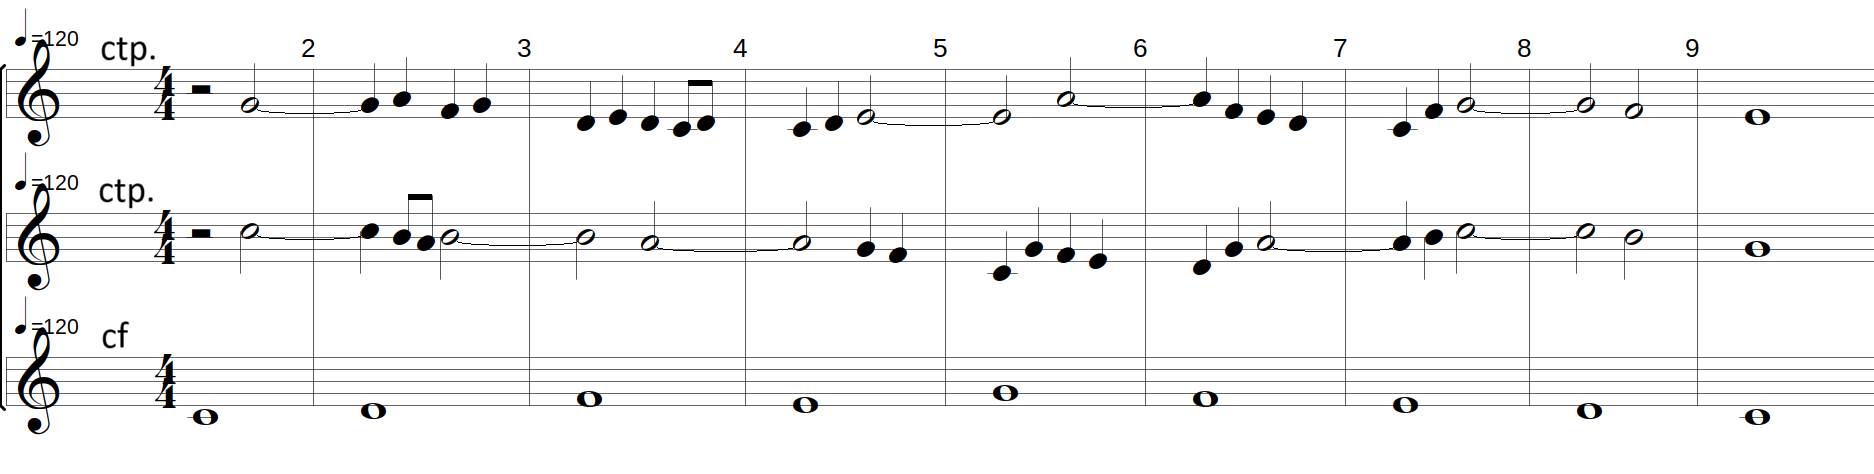
\includegraphics[width=1\textwidth]{Images/Experiments/basic-lexico-5sp.png}
    \caption{Result 5 of the lexicographic search method with default costs. Click \href{https://youtu.be/wYq28XcmpVw}{here} to listen.}
    \label{fig:lexico-5sp}
\end{figure}

Just as for the second experiment, some interesting things happen in the composition found by the lexicographic search. The intervals are more beautiful and the fact that there are dissonances that sometimes resolve gives more meaning to what's going on.

On the other hand, the fact that the penultimate note of the middle voice resolves on a G instead of a C is a bit frustrating, as the final chord feels like it is not a real ending, but this is a recurring problem in all solutions. The reason for this is probably that there is a rule (rule~\ref{rule:prefer-fifths-over-octaves}) that makes the solver prefer fifths to octaves, and there is no mention from Fux of deviating from this rule for the last measure.

\textit{However}, the solver did a surprisingly good job of finding passable solutions with such a small search field. The solutions obtained are far from high art, but you can see the musical intuition behind them.

\subsection{Mixing the technique of maximum minimisation with lexicographic order}\label{subsection:mixing-the-techniques}
Now what happens when we start to mix the techniques and group some of the costs in the lexicographic order? At each level of the lexicographic order, we calculate the maximum of the costs at that level, which we then try to minimise. All preferences that Fux has not explicitely ordered get packed on the same level, i.e. three levels subsist: the first one, with only the cost for successive perfect consonances, the second one, with only the cost for not using a harmonic triad, and a third one, with all the other costs.

\begin{figure}[h]
    \centering
    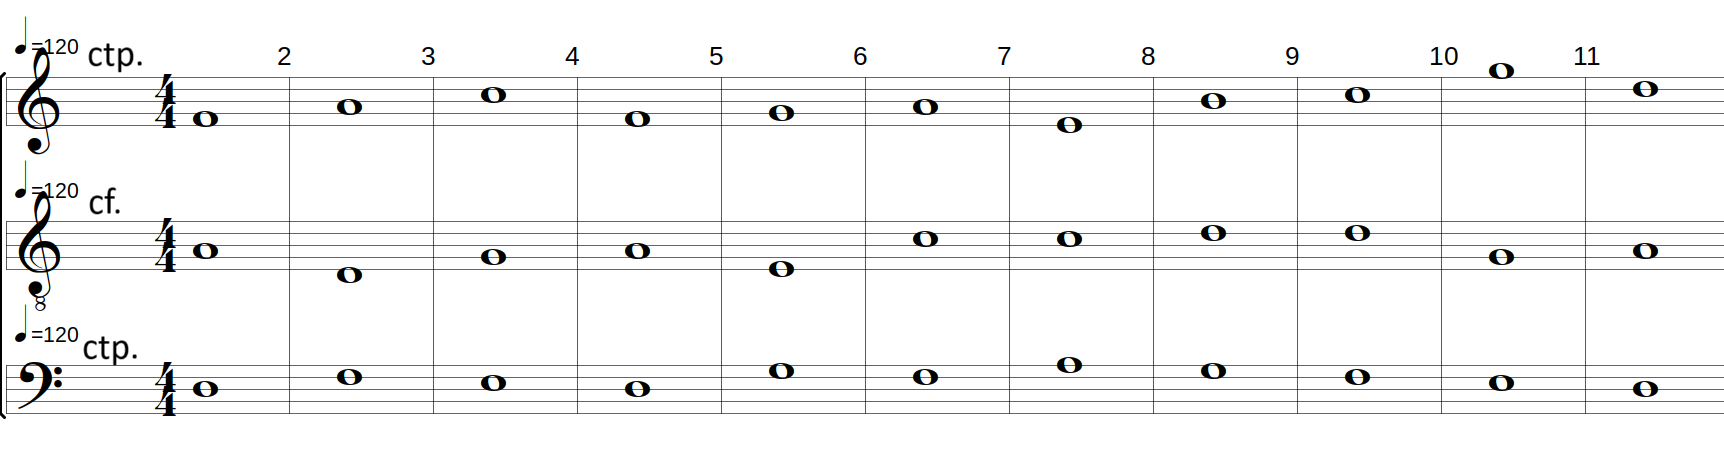
\includegraphics[width=1\textwidth]{Images/Experiments/min-1sp.png}
    \caption{Result 1 of a mix between lexicographic and maximum minimisation method. Click \href{https://example.com/}{here} to listen.}
    \label{fig:min-sp}
\end{figure} 
\begin{figure}[h]
    \centering
    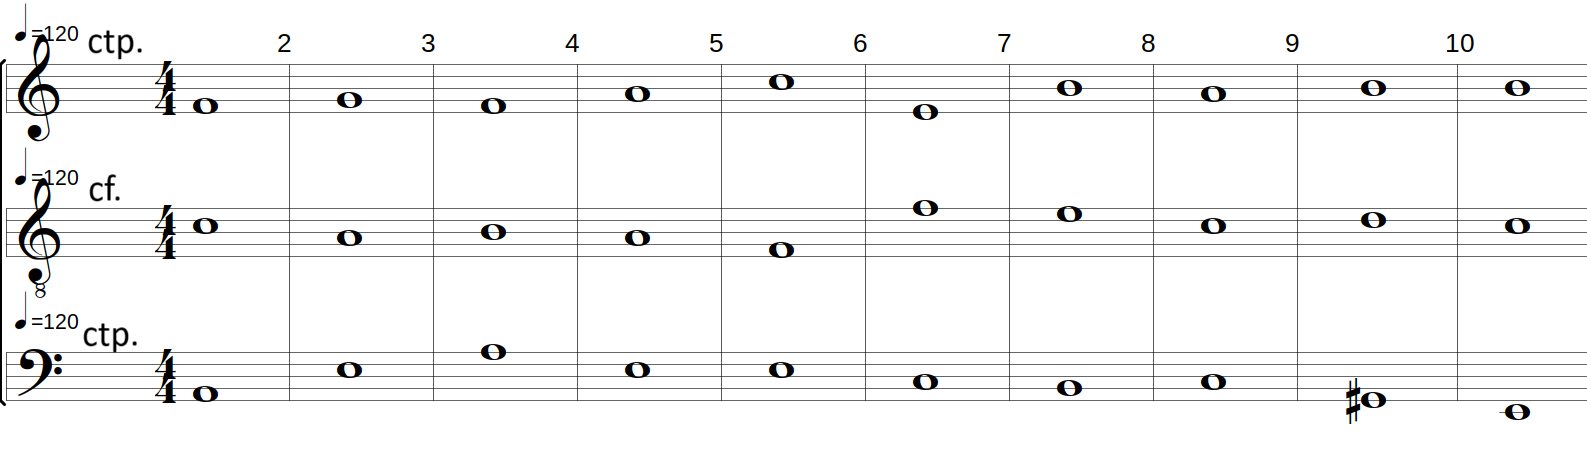
\includegraphics[width=1\textwidth]{Images/Experiments/min-1sp0.png}
    \caption{Result 2 of a mix between lexicographic and maximum minimisation method. Click \href{https://youtu.be/GRGE7NN3jNE}{here} to listen.}
    \label{fig:min-sp0}
\end{figure}

Figures~\ref{fig:min-sp} and~\ref{fig:min-sp0} show the solutions found by mixing the techniques of lexicographic order and maximum minimisation.

Both solutions handle the ending strangely, but this may be a coincidence, as there is no cost that would obviously cause such an ending.

It would be too bold to say that there is a big difference between the results obtained by this method and those obtained by the others. In other words, to the average ear, the solutions provided by this search technique are not significantly different from those provided by the other search methods.


The good news, however, is that the result, far from being excellent, is different. This means that a composer can set up the tool as they wish and get different results from one setup to another. They might start with the default settings and then change one parameter after another until they find what suits them best. This is really good news, because it means that the solution is not too limited to a few possibilities, but that once a valid solution has been found, there is still too much room for personalisation!


Note that the predicted bottleneck effect from section~\ref{section:minimising-the-maxima} was indeed observed in both searches, as the solution stopped improving after only ten seconds of search. After these ten seconds, the solver stopped finding better solutions because the third cost level (the one whose maximum was minimised) had already reached its minimum maximum, and so the solver could not distinguish between two solutions if they had the same maximum, since this search technique doesn't allow it. Please refer to figure~\ref{fig:bottleneck} for a better understanding of the situation.


\section{Conclusion on the search methods}
As we have stressed several times in this chapter, there is probably no \textit{best} way of ordering costs. Each technique has its shortcomings, and it is probably by allowing the composer to order their costs as they see fit that the tool will be able to reveal its full potential. 

Nevertheless, the lexicographic method seems capable of expressing more character than the cost soup of the linear combination method. The intransigent side of the lexicographic method can be adjusted by combining several costs at the same level of the lexicographic order. This combination can be achieved using the method of minimising maxima, but it should be noted that this is only possible to a certain extent if we want to avoid a cost creating a bottleneck on its own. It may also be preferable to combine costs at one level of the lexicographic order by simple addition, at the risk of making certain costs at that level explode.
The best compromise that has been found is therefore to give the composer as much choice as possible, by offering them the three possibilities, as well as the combination between the lexicographical order and the other two techniques. This allows the composer to compose their counterpoint iteratively: they make a first attempt that doesn't work well, adjust the costs to direct the search, and so on, until they gets the result that suits them best. In practice, this leads to the user interface described in Appendix~\ref{chapter:user-guide}, where a composer can choose their preferred preference order of importance (lexicographic order), then choose if they prefear the costs to be combined in a linear combination or maximum minimisation fashion.

